% This is samplepaper.tex, a sample chapter demonstrating the
% LLNCS macro package for Springer Computer Science proceedings;
% Version 2.21 of 2022/01/12
%
\documentclass[runningheads]{llncs}
\usepackage[T1]{fontenc}
% T1 fonts will be used to generate the final print and online PDFs,
% so please use T1 fonts in your manuscript whenever possible.
% Other font encondings may result in incorrect characters.
%
\usepackage{graphicx}
\usepackage{multirow}
\usepackage{floatrow}  
\usepackage{paralist}     % provides compactitem, a more compact itemize
% Used for displaying a sample figure. If possible, figure files should
% be included in EPS format.
%
% If you use the hyperref package, please uncomment the following two lines
% to display URLs in blue roman font according to Springer's eBook style:
\usepackage{hyperref}
\usepackage{booktabs}
\usepackage{tikz}
\usepackage{color}
\renewcommand\UrlFont{\color{blue}\rmfamily}

% other packages
\usepackage[noend,linesnumbered]{algorithm2e}
\usepackage{amsmath}
%\usepackage{subfloat}
\usepackage{csquotes}
\usepackage{todonotes}
\usepackage{subcaption}
% other files to include

% define your own macros here
\newcommand{\singlePrec} {\ensuremath{\mathit{ \mathord{\prec} }}}
\newcommand{\tasks} {\ensuremath{\mathit{tasks}}}

\newcommand{\GetPreEff} {\ensuremath{\mathit{GetPreEff}}}
\newcommand{\visited} {\ensuremath{\mathit{visited}}}

\newcommand{\matha} {\ensuremath{\mathit{a}}}
\newcommand{\mathb} {\ensuremath{\mathit{b}}}
\newcommand{\mathc} {\ensuremath{\mathit{c}}}

\newcommand{\Eff} {\ensuremath{\mathit{eff}}}  % example command without arguments
\newcommand{\Pre} {\ensuremath{\mathit{pre}}}  % (again)
\newcommand{\Add} {\ensuremath{\mathit{add}}}
\newcommand{\Del} {\ensuremath{\mathit{del}}}
\newcommand{\PreS} {\ensuremath{\mathit{pre^{*}}}}
\newcommand{\AddS} {\ensuremath{\mathit{add^{*}}}}
\newcommand{\DelS} {\ensuremath{\mathit{del^{*}}}}

\newcommand{\EffPlus} {\ensuremath{\mathit{eff^{+}_{*}}}}
\newcommand{\EffMinus} {\ensuremath{\mathit{eff^{-}_{*}}}}
\newcommand{\PossEffPlus} {\ensuremath{\mathit{poss-eff^{+}_{*}}}}
\newcommand{\PossEffMinus} {\ensuremath{\mathit{poss-eff^{-}_{*}}}}

\newcommand{\RelEffPlus} {\ensuremath{\mathit{eff^{\emptyset +}_{*}}}}
\newcommand{\RelEffMinus} {\ensuremath{\mathit{eff^{\emptyset -}_{*}}}}
\newcommand{\RelPossEffPlus} {\ensuremath{\mathit{poss-eff^{\emptyset +}_{*}}}}
\newcommand{\RelPossEffMinus} {\ensuremath{\mathit{poss-eff^{\emptyset -}_{*}}}}
	
\SetKwRepeat{Do}{do}{while}
% \newtheorem{theorem}{Theorem}

% Note that you can easily specify arguments:
% \newcommand{\someMacro}[2] {Argument 1: #1, Argument 2: #2} % example command with two arguments
% you use it via \someMacro{Hello}{World!}

\setuptodonotes{fancyline, color=green!40} 

% \captionsetup{width=1.5\linewidth} 
% \subcaptionsetup{width=1.5\linewidth} 		

\begin{document}

\title{Finding Solution Preserving Linearizations For Partially Ordered Hierarchical Planning Problems}
\titlerunning{Solution Preserving Linearizations}
% If the paper title is too long for the running head, you can set
% an abbreviated paper title here

% \author{Anonymous}
\author{Ying Xian Wu\inst{1} \and
Songtuan Lin \inst{1} \and
Gregor Behnke\inst{2} \and
Pascal Bercher\inst{1} }

%\authorrunning{Wu. Y et al.}
% First names are abbreviated in the running head.
% If there are more than two authors, 'et al.' is used.
%
\institute{
	School of Computing, The Australian National University, Canberra, Australia\inst{1}\\
	ILLC, University of Amsterdam, Amsterdam, The Netherlands\inst{2}\\
	\email{ \{yingxian.wu, songtuan.lin, pascal.bercher\}@anu.edu.au, g.behnke@uva.ni}
}


%\email{\{abc,lncs\}@uni-heidelberg.de}}
%
\maketitle              % typeset the header of the contribution
%
\begin{abstract}
Solving partially ordered hierarchical planning problems is more computationally expensive compared to solving totally ordered ones. Therefore, automatically transforming partially ordered problem domains into totally ordered ones, such that the totally ordered problem still retains at least one solution, would be a desired capability as it would reduce complexity and thus make it easier for planning systems to solve the problem. This is a complex endeavour, because even creating \emph{all} possible linearizations of all methods in the original domain does not guarantee that solutions are preserved. 
It also allows the planner to use algorithms and heuristics specialised for the totally ordered case to solve the transformed problem. 
In this paper, we propose an algorithm for converting partially ordered problems into totally ordered ones and give criterion for when this is possible. We test our techniques on the partially-ordered track of the bench-mark set of the IPC 2020 and solve both the linearized and the original partially-ordered problems using state-of-the-art planning systems. We find that in the majority of problems across a variety of domains, the linearized problem remains solvable, and can always be solved faster than the without our proposed pre-processing technique.

\keywords{Partially ordered HTN planning \and  Hierarchical planning \and Totally ordered HTN planning }
\end{abstract}
 
 
 
\section{Introduction}
Hierarchical Task Network (HTN) planning \cite{HTNSurvey} \cite{IntroGhallab} is a hierarchical approach to planning. Tasks in HTN planning are either primitive, corresponding to an action that can be taken, or compound. HTN problems have a set of methods that specify how one might achieve a given compound task, by decomposing it into a set of sub-tasks. A compound task may even decompose into itself, either directly via a method, or indirectly via a sequence of method applications. If decomposition leads to a sequence of primitive tasks executable from the initial state, then this sequence of actions is a solution to the problem, also known as a \enquote{plan}.

In totally ordered HTN planning, or TOHTN planning, methods specify a total order on the sub-tasks. In partially ordered HTN planning, or POHTN planning, methods might only specify a partial order on the sub-tasks. 

%Existing problems must be modelled in HTN planning formalism in order to be solved by %existing planners, but the order in which tasks can be done is often unknown.
%This observation the forms the basis -- if a partially ordered problem could be quickly and %automatically analysed, then reduced to a decidable form without losing all solutions.

Certain kinds of problems might be naturally more suited to being modelled as a partially ordered problem, for example, the actions \enquote{deliver package 1 to city A} and \enquote{deliver package 2 to city B} -- these are essentially unrelated goals in a real transport scenario, and so modelling the problem to require that one task be completed before the other would be unnecessarily limiting the possible solution space. In some cases, such over-specification may remove all valid solutions. Thus many problems might be \emph{modelled} as POHTN problems. However, for \emph{solving} the problem, it is desirable to have additional constraints that reduces the search space, while still preserving at least some of the actual solutions.

This paper specifically presents a method to transform a POHTN problem to a TOHTN problem in order to reduce the search space. Converting the problem to a TOHTN problem allows us to exploit the fact that as proven in Erol et al.\ \cite{ErolHTNExpressivity},  TOHTN planning as a class of problems has lower computational complexity, resulting in lower worst-case solving time. 
Thus, transforming a POHTN problem to a TOHTN problem could allow us to solve the problem more quickly and deploy specialised algorithms and heuristics.

The drawback to this approach is that, due to the greater expressivity of POHTN planning, there may exist POHTN problems that cannot be solved when converted to a TOHTN problem. For example, Erol et al.\ \cite{ErolHTNExpressivity} proved that HTN planning is expressive enough to model undecidable problems, such as the language intersection problem of two context-free languages. Fortunately, not every POHTN problem is guaranteed to be undecidable, and so could still be transformed while preserving at least one solution.

% This is beneficial because heuristic design is comparably easy for total-order problems due to the missing interaction between tasks. Also, we get another class of decidable partially ordered problems that's orthogonal to recursive ones. 

% Also, the domain model might be more intuitive: if a task is independent of some others it might be counter-intuitive to demand a certain position of it (if artificially made totally ordered). Plan recognition: independent goals can be described in parallel with POHTN planning but not with TOHTN \cite{DanielPlanRecognition}.

%\subsubsection{Contributions}
In this paper we present and investigate an algorithm for converting POHTN problems to TOHTN problems. We prove that when certain criteria are met, it guarantees that at least one solution will be preserved. 
Also, we obtain a new class of decidable problems, namely those that satisfy the above mentioned criterion. Finally, we show that, even when these criteria are not met, very few problems are rendered unsolvable by the transformation, and that it greatly reduces solving time for problems, with gains being bigger for more difficult problems. 



\section{Hierarchical Planning}
We first introduce classical planning, as hierarchical
planning can be considered an extension of classical planning.

\subsection{Planning Problem Formalisation}
Classical planning problems are defined over a \textbf{domain D} = $(F, A)$, where 
$F$ is a finite set of facts, or propositional state variables.
$A$ is a finite set of actions. 
For all $a \in A$,  $a \in 2^F \times 2^F \times 2^F$, which represents the preconditions and add and delete effects of an action. %$\langle pre, add, del \rangle$. 
The preconditions, add, and delete effects, of an action $a$ are referred to as $\Pre(a), \Add(a)$, and $\Del(a)$ respectively.
An action $a$ is executable in a state $s$ if its precondition $pre$ holds in $s$, i.e. $pre \subseteq s$. 
If executable in $s$, its result is the successor state $s'$ = $(s \backslash \Del) \cup \Add$, i.e., variables in $\Del(a)$ get removed and variables in $\Add(a)$ get added.

A \textbf{classical planning problem} is defined as $\textbf{P} = (D, S_I, S_G)$, 
where $D$ is the domain of the problem, 
$S_I \in 2^F$ is the initial state and $S_G \in F$ is the goal description.
Given a state $s \in 2^F$ , a fact is known for certain to be either true or false, i.e. information about the world state is complete at all times (this is called the closed world assumption).

A \textbf{solution} $\bar{a}$ to a problem is any action sequence that is executable in the initial state $S_I$, and leads to a state $s''$ that satisfies all
goals, i.e., $s'' \supseteq S_G$. Any such state $s''$ is called a goal state.


There are many formalisations for hierarchical planning, also known as \textbf{HTN planning}. The following one borrows heavily from Bercher et al.\ \cite{HTNSurvey} and Geier and Bercher \cite{Geier2011TIHTNDecidability}. HTN planning has two variants, Partially Ordered Hierarchical Task Network Planning, also known as POHTN planning, and Totally Ordered Hierarchical Planning, also called TOHTN planning,   % except with the initial task network replaced by a initial compound task. 

A POHTN problem \textbf{P} = $(D, S_I, T_I)$
is defined over some domain $D$, 
has an initial state $S_I \in 2^F$, and 
has a initial compound task $T_I$. 
The closed world assumption also holds for HTN planning.

The domain \textbf{D} = $(F, T_P, T_C, \delta, M)$, where
$F$ is the finite set of facts or state variables, $T_P$ is the finite set of all possible primitive task names, $T_C$ is the finite set of all possible compound task names, and
$\delta$ is a mapping from primitive task name to action. Actions in POHTN domain also have preconditions, adds, and delete effects.
$M$ is the finite set of decomposition methods. Each one maps a compound task name to a task network. If $m \in M$, then $m=(c, tn)$, where $c \in T_C$.

A task network \textbf{tn} = $(T, \singlePrec, \alpha)$ consists of
T, which is a finite set of task identifiers (ids); 
$\singlePrec$, which is a partial order over T; and
$\alpha$, which maps task ids $\in$ T to task names in $T_C$ and $T_P$. 

% replacing t  (i.e. $tn_1 \rightarrow_{t,m} tn_2$)
A method $m$ decomposes a task network $tn_1 = (T_1, \singlePrec_1, \alpha_1)$ into
a new task network $tn_2$ by replacing $t$, if and only if $t \in T_1$, $\alpha_1(t) = c$, and $\exists tn' = (T', \singlePrec' \alpha')$ with $tn' \cong tn_m$ and $T' \cap T = \emptyset$ and
\begin{align}
tn_2 :=     &((T_1 \setminus \{t\}) \cup T',    \singlePrec_1 \cup \singlePrec' \cup \singlePrec_X,        \alpha_1 \cup \alpha') \\
\singlePrec_X :=  &\{(t_1, t_2) \in T_1 \times T'  \mid  (t_1,t) \in \singlePrec_1 \} \cup \\
&\{(t_1, t_2) \in T' \times T_1 \mid (t, t_2) \in \singlePrec_1 \}  
\end{align}
In other words, the decomposition of a compound task results in it being removed from the task network and replaced by a copy of the method’s task network. The ordering constraints
on the removed task are inherited by its replacement tasks, as defined by $\singlePrec_X$. 

A solution to an HTN problem is a task network $tn = (T, \prec, \alpha)$ if and only if
tn can be reached via decomposing $tn_I$, all tasks are primitive, ($\forall t \in T: \alpha(t) \in T_P$), and there exists a sequence $\langle t_1, t_2 ... t_n \rangle$ of the task ids in $T$ that agrees with $\prec$ such that the application of that sequence $\langle \alpha(t_1), \alpha(t_2) ... \alpha(t_n) \rangle$ in $S_I$ is executable.
     
In other words, the goal of hierarchical planning is to find an decomposition of the task, then any executable refinement of the resulting decomposition. Whereas in classical planning, one only finds any executable sequence of actions to achieve a goal state, so HTN planning poses additional restrictions on which action sequences may be considered.

\textbf{Totally Ordered Hierarchical Planning}, also called TOHTN planning, is the same as partially ordered planning in all respects except the kind of task networks it allows.
For both planning formalisms, a method $m$ maps a task $t$ to a task network \textbf{tn} = $(T, \prec, \alpha)$. TO planning domains require that $\prec$ must specify a total order between task ids in $T$.
This leads to a difference in expressiveness and decide-ability of TOHTN vs POHTN planning. POHTN planning is more expressive in general (both in terms of plan existence and in terms of computational complexity). As per H\"{o}ller et al.\ \cite{LanguageClassificationPlanning}, if regarded from the standpoint of formal grammars, TO planning is exactly as expressive as context free languages, whereas PO planning is strictly more expressive than context-free languages, and strictly less expressive than context-sensitive languages.
In terms of complexity classes, Erol et al.\ \cite{ErolHTNExpressivity} proved that POHTN planning is semi-decidable, whereas
Alford et al.\ \cite{Alford2015TightHTNBounds} proved that, assuming arbitrary recursion, TOHTN planning is 2-EXPTIME-complete with variables, and EXPTIME-complete without. 

 
%\textbf{Tail-recursive problems} are HTN problems where methods can only recurse through the last task in their task network. Problems that don't have recursion are also tail-recursive. \cite{Alford2015TightHTNBounds}

%\todo{maybe rephrase it a little bit? there are a lot of stuffs between decidable and undecidable problems}% Relying on a comparison to the Chomsky hierarchy, H\"{o}ller et al. [2014;2016] conducted an in-depth  showing which problems (i.e., which intended solution sets) can be expressed by various hierarchical and non-hierarchical formalisms. 

%\subsubsection{Grammars}
%The following explanation for \cite{ChomskyHeirarchyRogers}
%A grammar $G$ is defined as $(N, \epsilon, P, S)$, where
%$N$ is  a set of non-terminal symbols, 
%$\epsilon$ is a set of terminal symbols,
%$P$ a set of production rules, that maps elements in $N$ to a finite sequence of elements in %$\epsilon$
%$S$ is the start symbol.
%A $Language$, defined by a specific grammar $G$, consists of all strings that can be produced by repeated application, including infinite applications, of the production rules to the start symbol $S$.

%In a context-free grammar, all production rules $\in P$ take the form $A \implies b$ where $A$ is a single non-terminal symbol and $b$ is a string of symbols. CFLs are those languages that %can be defined by a context-free grammar.

%The Chomsky hierarchy defined a relationship between these different classes of grammars, based off whether one grammar can pruduce all possible languages possible using another grammar class. Context-sensitive grammars are more general than context-free grammars, in the sense that there are languages that can be described by CSG but not by context-free grammars.
 
\section{Linearization Method}

Though this will not always be possible, we want to impose a total order on the task networks, such that for a method $m = (c, (T, \singlePrec, \alpha))$, the decomposition of $t$ will result in an executable sequence. To attempt this, one could analyse what preconditions the execution of sub-tasks in $T$ might need, and what effects they might have. For example, if a sub-task $t$ deletes a fact in the precondition for sub-task $t'$, one could order $t'$ before $t$ to avoid invalidating the precondition for $t'$. So we need a way of estimating preconditions and effects for compound tasks. It was proven by Olz et al.\ \cite{ConnyPreEstimation} that inferring all preconditions and effects of a compound task is as difficult as solving the problem. Therefore, a polynomial-time algorithm to infer the exact set of preconditions and effects of a compound task does not exist. However, using an approximated set, one can analyse the proposed orderings and resolve any conflicts, e.g. cycles. If conflict-resolution is necessary, we refer to this as needing \textbf{\textit{cycle-breaking}}.

The algorithm provided in this paper approximates possible preconditions and effects for all tasks so that this information can be used to linearize methods. 
For a given task $t$, we  call these approximate preconditions and effects as $\PreS(t), \DelS(t), \AddS(t)$.
If t is an action, $\PreS(t), \DelS(t), \AddS(t)$ is the same as $\Pre(t), \Add(t), \Del(t)$. 
If t is a compound task, $\PreS(t)$, $\AddS(t),  \DelS(t)$, are the union of the respective preconditions, add, and delete effects of all actions that $t$ could decompose to, as shown in Figure~\ref{CompoundPreEff}.
This means that for a task $t$ $\PreS(t), \DelS(t), \AddS(t)$ can contain contradictory effects, e.g. $t$ adds \emph{and} deletes a fact. These are essentially the mentioned literals defined by de Silva et al.\ \cite{mentionedliterals}.

Figure~\ref{AddOrderings} shows how the additional orderings for a method are determined. We then attempt to integrate these orderings into the method $m = (t, (T, \singlePrec, \alpha))$. If there exists a cycle after integrating the new orderings into $\singlePrec$, we remove a random one of the new orderings in that cycle, as shown in Figure~\ref{CycleBreak}, until that cycle no longer exists.
We repeat this for all methods in order to linearize them.

\begin{figure}
	\scalebox{0.8} {
	\begin{subfigure}{5cm}
		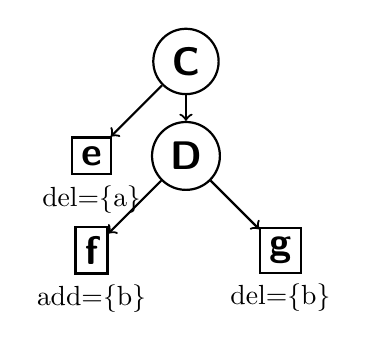
\begin{tikzpicture}[->,auto,node distance=1.2cm,
		thick,main node/.style={circle,draw,font=\sffamily\Large\bfseries},
		square effect/.style={rectangle,draw,font=\sffamily\Large\bfseries}]
		
		\node[main node] (1) {C};
		\node[main node] (2) [below of=1] {D};
		\node[square effect, label=below:{del=\{a\}}] (3) [below of=2, left of=1] {e};
		\node[square effect, label=below:{add=\{b\}}] (4) [below of=2, left of=2] {f};
		\node[square effect, label=below:{del=\{b\}}] (5) [below of=2, right of=2] {g};
		
		\path[every node/.style={font=\sffamily\small}]
		(1) edge node [right] {} (2)
		(1) edge node [right] {} (3)
		(2) edge node [right] {} (4)	
		(2) edge node [right] {} (5);
		\end{tikzpicture}
	\end{subfigure}
}
	\hspace{1cm}
\scalebox{0.8}{
	\begin{subfigure}{3cm}
		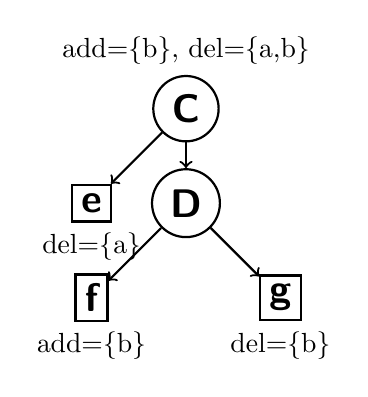
\begin{tikzpicture}[->,auto,node distance=1.2cm,
		thick,main node/.style={circle,draw,font=\sffamily\Large\bfseries},
		square effect/.style={rectangle,draw,font=\sffamily\Large\bfseries}]
		
		\node[main node, label={add=\{b\}, del=\{a,b\}} ] (1) {C};
		\node[main node] (2) [below of=1] {D};
		\node[square effect, label=below:{del=\{a\}}] (3) [below of=2, left of=1] {e};
		\node[square effect, label=below:{add=\{b\}}] (4) [below of=2, left of=2] {f};
		\node[square effect, label=below:{del=\{b\}}] (5) [below of=2, right of=2] {g};
		
		\path[every node/.style={font=\sffamily\small}]
		(1) edge node [right] {} (2)
		(1) edge node [right] {} (3)
		(2) edge node [right] {} (4)	
		(2) edge node [right] {} (5);
		\end{tikzpicture}   
	\end{subfigure} 
}
	\caption{Inferring preconditions and effects for compound tasks}
	\label{CompoundPreEff}
\end{figure}

\begin{figure}
	\scalebox{0.8}{
	\begin{subfigure}{5cm} 
		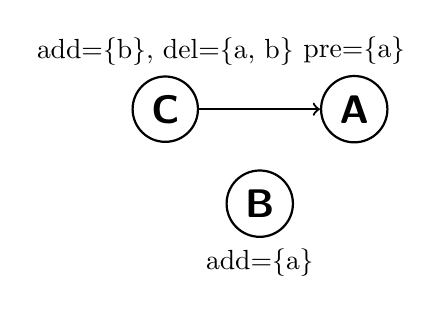
\begin{tikzpicture}[->,auto,node distance=1.2cm,
		thick,main node/.style={circle,draw,font=\sffamily\Large\bfseries},
		square effect/.style={rectangle,draw,font=\sffamily\Large\bfseries}]		
		\node[main node, label={add=\{b\}, del=\{a, b\}}] (3) {C};
		\node[main node, label=below:{add=\{a\}}] (2) [right of=3, below of=3] {B};
		\node[main node, label={pre=\{a\}}] (1) [right of=2, above of=2]  {A};		

		\path[every node/.style={font=\sffamily\small}]
		(3) edge node [left] {} (1);
		\end{tikzpicture}
		\caption{The original method}
	\end{subfigure}
}
	\hspace{1cm}	
\scalebox{0.8}{
		\begin{subfigure}{5cm}
		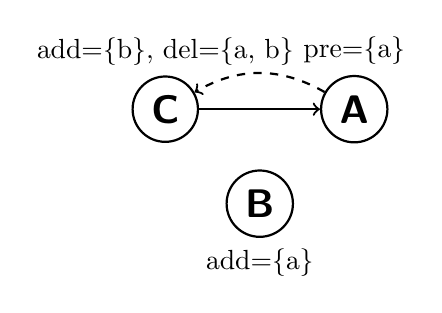
\begin{tikzpicture}[->,auto,node distance=1.2cm,
		thick,main node/.style={circle,draw,font=\sffamily\Large\bfseries},
		square effect/.style={rectangle,draw,font=\sffamily\Large\bfseries}]

		\node[main node, label={add=\{b\}, del=\{a, b\}}] (3) {C};
		\node[main node, label=below:{add=\{a\}}] (2) [right of=3, below of=3] {B};
		\node[main node, label={pre=\{a\}}] (1) [right of=2, above of=2]  {A};
		
		\path[every node/.style={font=\sffamily\small}]
		(1) edge[dashed, bend right] node [left] {} (3)
		(3) edge node [left] {} (1);
		\end{tikzpicture}
		 \caption{C deletes a fact (a) that is in preconditions for A  -- so A is ordered before C}
	\end{subfigure}
}
	\vspace{2em}
	\scalebox{0.8}{
	\begin{subfigure}{5cm}
		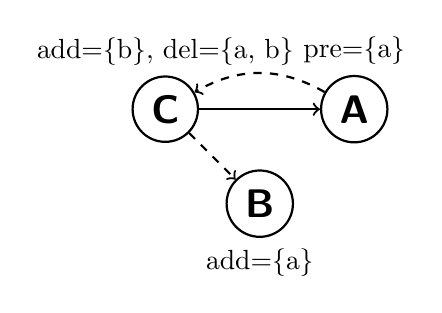
\begin{tikzpicture}[->,auto,node distance=1.2cm,
		thick,main node/.style={circle,draw,font=\sffamily\Large\bfseries},
		square effect/.style={rectangle,draw,font=\sffamily\Large\bfseries}]
			
		\node[main node, label={add=\{b\}, del=\{a, b\}}] (3) {C};
		\node[main node, label=below:{add=\{a\}}] (2) [right of=3, below of=3] {B};
		\node[main node, label={pre=\{a\}}] (1) [right of=2, above of=2]  {A};
					
		\path[every node/.style={font=\sffamily\small}]
		(3) edge[dashed] node [right] {} (2)
		(1) edge[dashed, bend right] node [left] {} (3)
		(3) edge node [left] {} (1);
		\end{tikzpicture}
		\caption{B adds a fact (a) that C deletes -- so C is ordered before B}
	\end{subfigure}
}
	\hspace{1cm}
	\scalebox{0.8}{
	\begin{subfigure}{5cm}
		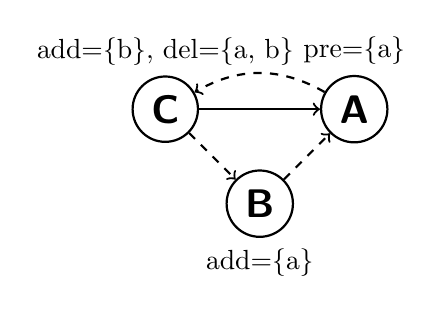
\begin{tikzpicture}[->,auto,node distance=1.2cm,
		thick,main node/.style={circle,draw,font=\sffamily\Large\bfseries},
		square effect/.style={rectangle,draw,font=\sffamily\Large\bfseries}]
		
		\node[main node, label={add=\{b\}, del=\{a, b\}}] (3) {C};
		\node[main node, label=below:{add=\{a\}}] (2) [right of=3, below of=3] {B};
		\node[main node, label={pre=\{a\}}] (1) [right of=2, above of=2]  {A};
		
		\path[every node/.style={font=\sffamily\small}]
		(2) edge[dashed] node [right] {} (1)
		(3) edge[dashed] node [right] {} (2)
		(1) edge[dashed, bend right] node [left] {} (3)
		(3) edge node [left] {} (1);
		\end{tikzpicture}
		\caption{B adds a fact (a) that is in preconditions for A -- so B is ordered before A}
	\end{subfigure}
}
	\caption{Adding possible orderings to methods}
	
	\label{AddOrderings} 
\end{figure}



\begin{figure}
	\begin{subfigure}{5cm}
		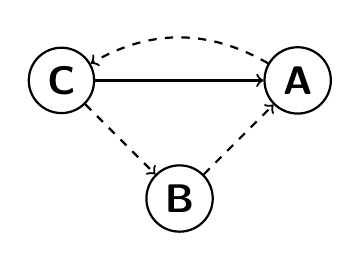
\begin{tikzpicture}[->,auto,node distance=1.5cm,
		thick,main node/.style={circle,draw,font=\sffamily\Large\bfseries},
		square effect/.style={rectangle,draw,font=\sffamily\Large\bfseries}]
		
		\node[main node] (3) {C};
		\node[main node] (2) [right of=3, below of=3] {B};
		\node[main node] (1) [right of=2, above of=2]  {A};
				
		\path[every node/.style={font=\sffamily\small}]
		(2) edge[dashed] node [right] {} (1)
		(3) edge[dashed] node [right] {} (2)
		(1) edge[dashed, bend right] node [left] {} (3)
		(3) edge node [left] {} (1);
		\end{tikzpicture}
		\caption{Perform depth-first search on the modified method}
	\end{subfigure}
	\hspace{1cm}
	\begin{subfigure}{5cm}
		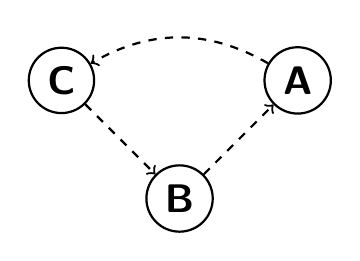
\begin{tikzpicture}[->,auto,node distance=1.5cm,
		thick,main node/.style={circle,draw,font=\sffamily\Large\bfseries},
		square effect/.style={rectangle,draw,font=\sffamily\Large\bfseries}]
		
		\node[main node] (3) {C};
		\node[main node] (2) [right of=3, below of=3] {B};
		\node[main node] (1) [right of=2, above of=2]  {A};
		
		\path[every node/.style={font=\sffamily\small}]
		(2) edge[dashed] node [right] {} (1)
		(3) edge[dashed] node [right] {} (2)
		(1) edge[dashed, bend right] node [left] {} (3);
		\end{tikzpicture}
		\caption{Identify cycle (path along which a node is reachable from one of their ancestors)}
	\end{subfigure}
	
	
	\begin{subfigure}{5cm}
		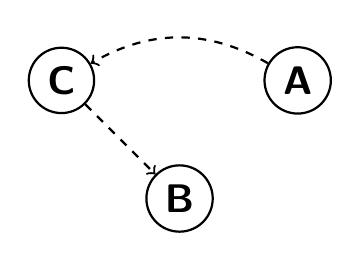
\begin{tikzpicture}[->,auto,node distance=1.5cm,
		thick,main node/.style={circle,draw,font=\sffamily\Large\bfseries},
		square effect/.style={rectangle,draw,font=\sffamily\Large\bfseries}]
		
		\node[main node] (3) {C};
		\node[main node] (2) [right of=3, below of=3] {B};
		\node[main node] (1) [right of=2, above of=2]  {A};
				
		\path[every node/.style={font=\sffamily\small}]
		%(2) edge[dashed] node [right] {} (1)
		(3) edge[dashed] node [right] {} (2)
		(1) edge[dashed, bend right] node [left] {} (3);
		\end{tikzpicture}
		\caption{Pick an edge not originally in the method (i.e. a dashed line edge) and delete it.}
	\end{subfigure}
	\hspace{1cm}
	\begin{subfigure}{5cm}
		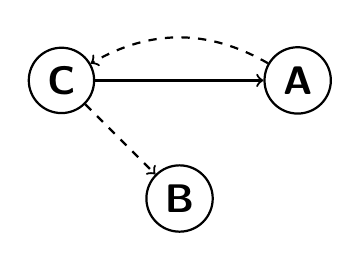
\begin{tikzpicture}[->,auto,node distance=1.5cm,
		thick,main node/.style={circle,draw,font=\sffamily\Large\bfseries},
		square effect/.style={rectangle,draw,font=\sffamily\Large\bfseries}]
		
		\node[main node] (3) {C};
		\node[main node] (2) [right of=3, below of=3] {B};
		\node[main node] (1) [right of=2, above of=2]  {A};
		
		\path[every node/.style={font=\sffamily\small}]
		%(2) edge[dashed] node [right] {} (1)
		(3) edge[dashed] node [right] {} (2)
		(1) edge[dashed, bend right] node [left] {} (3)
		(3) edge node [left] {} (1);
		\end{tikzpicture}
		\caption{Repeat as necessary until depth-first search cannot find any path back to a previously visited node}
	\end{subfigure}
	\vspace{2cm}
	
	\begin{subfigure}{5cm}
		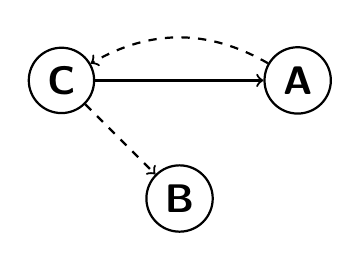
\begin{tikzpicture}[->,auto,node distance=1.5cm,
		thick,main node/.style={circle,draw,font=\sffamily\Large\bfseries},
		square effect/.style={rectangle,draw,font=\sffamily\Large\bfseries}]
		
		\node[main node] (3) {C};
		\node[main node] (2) [right of=3, below of=3] {B};
		\node[main node] (1) [right of=2, above of=2]  {A};
				
		\path[every node/.style={font=\sffamily\small}]
		%(2) edge[dashed] node [right] {} (1)
		(3) edge[dashed] node [right] {} (2)
		(1) edge[dashed, bend right] node [left] {} (3)
		(3) edge node [left] {} (1);
		\end{tikzpicture}
		\caption{Perform depth-first search on the modified method (again)}
	\end{subfigure}
	\hspace{1cm}
	\begin{subfigure}{5cm}
		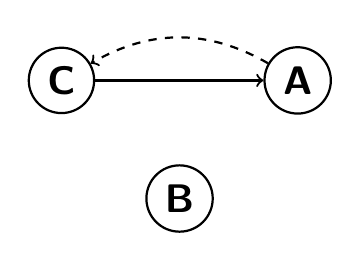
\begin{tikzpicture}[->,auto,node distance=1.5cm,
		thick,main node/.style={circle,draw,font=\sffamily\Large\bfseries},
		square effect/.style={rectangle,draw,font=\sffamily\Large\bfseries}]
		\node[main node] (3) {C};
		\node[main node] (2) [right of=3, below of=3] {B};
		\node[main node] (1) [right of=2, above of=2]  {A};
				
		\path[every node/.style={font=\sffamily\small}]
		%(2) edge[dashed] node [right] {} (1)
		%(3) edge[dashed] node [right] {} (2)
		(1) edge[dashed, bend right] node [left] {} (3)
		(3) edge node [left] {} (1);
		\end{tikzpicture}
		\caption{Identify cycle (path along which a node is reachable from one of their ancestors (again))}
	\end{subfigure}
	
	
	\begin{subfigure}{5cm}
		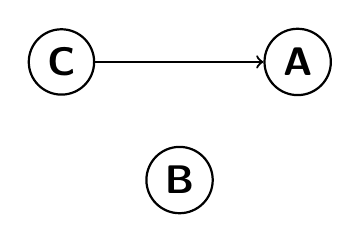
\begin{tikzpicture}[->,auto,node distance=1.5cm,
		thick,main node/.style={circle,draw,font=\sffamily\Large\bfseries},
		square effect/.style={rectangle,draw,font=\sffamily\Large\bfseries}]
		
		\node[main node] (3) {C};
		\node[main node] (2) [right of=3, below of=3] {B};
		\node[main node] (1) [right of=2, above of=2]  {A};
		
		\path[every node/.style={font=\sffamily\small}]
		%(2) edge[dashed] node [right] {} (1)
		%(3) edge[dashed] node [right] {} (2)
		%(1) edge[dashed, bend right] node [left] {} (3)
		(3) edge node [left] {} (1);
		\end{tikzpicture}
		\caption{Pick an edge not originally in the method (i.e. a dashed line edge) and delete it (again).}
	\end{subfigure}		
	\hspace{1cm}
	\begin{subfigure}{5cm}
		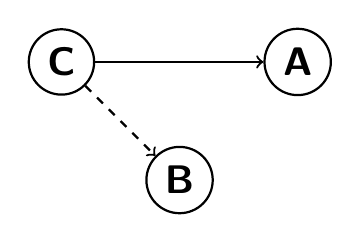
\begin{tikzpicture}[->,auto,node distance=1.5cm,
		thick,main node/.style={circle,draw,font=\sffamily\Large\bfseries},
		square effect/.style={rectangle,draw,font=\sffamily\Large\bfseries}]
		
		\node[main node] (3) {C};
		\node[main node] (2) [right of=3, below of=3] {B};
		\node[main node] (1) [right of=2, above of=2]  {A};
				
		\path[every node/.style={font=\sffamily\small}]
		%(2) edge[dashed] node [right] {} (1)
		(3) edge[dashed] node [right] {} (2)
		%(1) edge[dashed, bend right] node [left] {} (3)
		(3) edge node [left] {} (1);
		\end{tikzpicture}
		\caption{No more cycles, so perform a topological sort to produce a total ordering that satisfies the above constraints}
	\end{subfigure}	
	\caption{Cycle breaking to make method linearized}
	\label{CycleBreak} 
\end{figure}
 
 
\subsection{Code} 

\begin{align*}
& \forall t \in T_P : \PreS(t) = \Pre(t)  \land \AddS(t) = \Add(t)  \land \DelS(t) = \Del(t)  \\ %  \land
& \forall t \in T_C : \PreS(t) = \{f  \mid  \exists m \in M : m=(t,(T, \singlePrec, \alpha)) \forall t' \in T.  \forall  f \in \PreS(t') \}   \\
& \forall t \in T_C : \AddS(t) = \{f  \mid  \exists m \in M : m=(t,(T, \singlePrec, \alpha)) \forall t' \in T.  \forall  f \in \AddS(t') \}   \\
& \forall t \in T_C : \DelS(t) = \{f  \mid  \exists m \in M : m=(t,(T, \singlePrec, \alpha)) \forall t' \in T.  \forall  f \in \DelS(t') \}   \\
%& \forall t \in T_C : \PreS(t) = \{ \PreS(t)  \mid   \exists m \in M (m=(t,tn)) \}   \\
%& \forall t \in T_C : \DelS(t) = \{ \DelS(t)  \mid   \exists m \in M (m=(t,tn)) \}   \\
%& \forall t \in T_C : \AddS(t) = \{ \AddS(t)  \mid  \exists m \in M (m=(t,tn)) \}   \\
\end{align*}



\begin{algorithm}[H]\label{alg:Algorithm1}
	\KwData{$(F, T_P, T_C, \delta, M)$}
	\KwResult{$(F, T_P, T_C, \delta, M)$}
	
	%\For {c $\in$ $T_C$} {
	%	\PreS, \AddS, \DelS = GetPreEff($F, T_P, T_C, \delta, M, visited, m$)
	%}

	\For {$m=(t, (T_m, \singlePrec, \alpha)) \in M$}{  
		\tcc{An edge $(t, t')$ in $G$ means $t$ is ordered before $t'$}  
		$G \gets \singlePrec$ \\
		\For{a $\in$ F}{  
			\For{$t \in T_m$}{
				\For{$t' \in T_m$}{
					if $a \in \AddS(t)$ and $a \in \PreS(t')$, add $(t, t')$ to $G$  \\ 
					if $a \in \AddS(t)$ and $a \in \DelS(t')$, add $(t', t)$ to $G$  \\ 
					if $a \in \DelS(t)$ and $a \in \PreS(t')$, add $(t', t)$ to $G$  \\ 
					if $a \in \DelS(t)$ and $a \in \AddS(t')$, add $(t, t')$ to $G$ \\  
				}
			} 
		} 
		\While{$G$ has cycles in it}{
			Delete a random ordering in $G$ that is not in $\singlePrec$ \\   % $\PreS, \DelS, \AddS$, rather than $prec$ \;
		}
		$\prec'$ = Any linearization of $G$ \\
		$m' = (tasks(m), \prec', \alpha(t))$ \\
		$M' = M' \cup  \{m'\}$ \\
	}
	\Return $D' = (F, T_P, T_C, \delta, M')$ \\
	\caption{Calculation of linearized methods}
\end{algorithm}

 
\subsection{Runtime}

% One of main results is that one can find these linearizations in poly-time and that those remaining/found still solve the problem if it was solvable in the first place.
%I would see this as a theorem that requires two proofs:
%- the preservance of solutions of the technique (soundness)
%- the P-runtime.

%Could also be that this procedure takes exponential time, which would be much less impressive.

\begin{theorem}\label{thm:Runtime}
	Given a problem $P = (F, T_P, T_C, \delta, M)$, Algorithm~\ref{alg:Algorithm1} takes at most quadratic time, $\mathcal{O}( |M| * |F| * |T|^2)$. 
\end{theorem}
\begin{proof}  % ,  network of tasks it can decompose to as a tree of tasks whose edges are between a task and a task it can decompose to, since it excludes previously seen tasks. 
To calculate $\PreS, \AddS, \DelS$ for each task $t$, we can perform breadth-first search on the task decomposition sub-tree (where tasks are nodes, and edges indicate possible decomposition by methods) rooted at $t$. The size of a sub-tree has an upper limit of $T_C + T_P$ nodes. For each primitive task in the sub-tree, we can iterate over each fact to update $\PreS, \AddS, \DelS$ for the root $t$. Thus calculating  $\PreS, \AddS, \DelS$ for a single compound task has an upper limit of $(3 * |F| * |T_p|) + |T_C|$. This inference occurs for each compound task, so inference for all compound tasks takes $((3 * |F| * |T_p|) + |T_C|) * |T_C|$ time at most, or $\mathcal{O}(|F| * |T|^2)$, where $|T|$ refers to $|T_P| + |T_C|$.

% Note that actually visiting $T_c$ nodes for each method requires that the domain have the initial task as the only compound task. In practice, most problems are likely to have significant depth, so a method is likely to have significantly less than all tasks to explore.
%For the computation of $\PreS, \AddS, \DelS $, it is trivial to see that exploring the Task %Decomposition Tree (TDT) for all methods that can decompose a compound task $c$ allows you to infer %preconditions and effects of $c$. Let the function for this procedure be called GetPreEff($F, T_P, %T_C, \delta, M, visited, m$). Tasks form the nodes of this TDT, 
%the upper bound is M * log(T) * F
%\todo{define TDT}

Lines 5 to 12 of Algorithm~\ref{alg:Algorithm1} builds a graph to represent each method. This graph's nodes are tasks of the task network produced, and the edges represent orderings between tasks. The code here iterates over every method, which iterates over every fact, which iterates over every sub-task in that method, which iterates over every other sub-task in that method. Leading to $(M * F * (t_m)^2)$, where $t_m$ is the average number of sub-tasks per method. So it's at most $\mathcal{O}(|M| * |F| * |T|^2)$, since $t_m$ has an upper bound of $T$, where $T=T_p + T_C$.

Lines 12-13 of Algorithm~\ref{alg:Algorithm1} can be done by Depth-First Search (DFS). If a \enquote{back-edge}, defined as the edge that leads back to an already visited node (indicating a loop), then this edge is deleted, providing it was not part of the original domain. If it was part of the original domain, then assuming that the back edge was from node A to B, then a random edge is selected along any path from B to A (i.e. from the other part of the loop) and deleted instead.
DFS is known to be in $\mathcal{O}(|V|)$, and finding a path back can be achieved using Dijkstra's algorithm, which is known to be in $\mathcal{O}(|V|^2)$.
 
Temporal complexity of removing cycles is therefore $(|M| * ((t_m + t_m^2) * c)) = M * {t_m}^2 * c$, where $t_m$ is the number of sub-tasks produced by a method, and $c$ is the number of cycles.
% In practice, $c$ and $t_m$ will usually be small. 
This is approximately $\mathcal{O}(M * T^2 * c)$, since $t_m$ is upper bounded by $T$, where $T=T_p + T_C$.

Line 14 can be done via topological sort of the graph (which is known to be in $\mathcal{O}(V+E)$ in time and $\mathcal{O}(V)$ in space). In this case, the nodes of the graph are tasks, and the edges are orderings. So that's $M * (t_m+e_m)$, where $e_m$ is the number of \enquote{edges} in the new method, and has an upper bound of $e_m$ to find a topological sort for the sub-tasks of every method. That's approximately $\mathcal{O}(|M| * |T|)$, since both $t_m$ and $t_e$ are upper bounded by $T$, such that $T=T_p + T_C$.

So in total the main algorithm takes: \newline
$(|M| * |F| * |T|))$  +    % GetPreEff
$(|M| * |F| * |T|^2)$ + % Build new Graph
$(|M| * |T|^2 * c)$ +   % remove cycles
$(|M| * |T|))$        % topological sort
 

The number of times we need to remove an edge in a cycle, $c$, has an upper limit of $|F|$.
Adding an additional ordering (which may cause a cycle) requires interaction, and removing the aforementioned additional ordering will remove the cycle. Thus the maximum run-time of this algorithm is in $\mathcal{O}(M * F * T^2)$, i.e. quadratic time at most.
\end{proof}


\subsection{Theoretical properties}
\begin{theorem}\label{thm:Soundness}
	Given a POHTN planning problem $P$ and TOHTN problem
	$P'$ obtained from $P$ by using Algorithm~\ref{alg:Algorithm1}
	then the solution set of $P'$ is a not necessarily strict subset of that of $P$.
\end{theorem}
\begin{proof}
	The new desired orderings for a method include all of the orderings already required by the method originally. The algorithm then turns the tasks and new desired orderings between them into a directed graph, and the new ordering is produced by performing a topological sort on the nodes of that graph. This means we do not modify the sub-tasks a method produces, just the ordering between them, so the set of plans from the totally ordered method is just a subset of the plans possible from the partially ordered one. Any solution to the linearized problem is then obviously a solution to the original problem.
	\qed
\end{proof}

 
\begin{theorem}\label{thm:notCompleteness}
	Given a POHTN planning problem $P$ and TOHTN problem
	$P'$ obtained from $P$ by using Algorithm~\ref{alg:Algorithm1}
	then the solution set of $P'$ may be empty.
\end{theorem}
\begin{proof}
	This algorithm linearizes all the methods to be totally ordered. Since sub-tasks inherit the orderings of their parents, it's impossible to preserve a solution that requires the interleaving of sub-tasks if their respective parents that are already ordered with respect to each other. This proves that the algorithm can remove some possible action sequences, assuming the original domain was not already totally ordered. Consider the simple example problem:
	
	\begin{figure}
		\caption{Diagram showing an example problem and its decomposition.}		
		\begin{subfigure}{3.5cm}
			\begin{align*}
				F   = & \{a, b, c \}           \\
				N_p =  & \{A, B, C\}      \\
				N_c = & \{AC, T_I\}            \\ 
				M   = & \{  (T_I, \{AC, B\}), \\
				       &    (AC, \{A, C\})  \} \\
				 S_I = & \{ a \} 	             \\ 
			\end{align*} 
		\end{subfigure}		
		\scalebox{0.7}{
		\begin{subfigure}{7cm}
			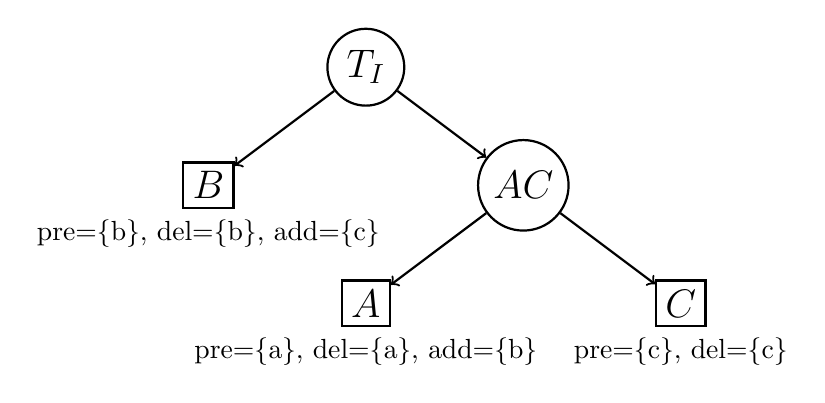
\begin{tikzpicture}[->,auto,node distance=1.5cm,
			thick,main node/.style={circle,draw,font=\sffamily\Large\bfseries},
			square node/.style={rectangle,draw,font=\sffamily\Large\bfseries}]
			\node[] (InitState) {}; %{ $\mathbf{S_I = \{a\}}$ };
					
			\node[main node] (Init) [right=3cm of InitState] {$T_I$};
			\node[main node] (AC) [right=2cm of Init, below of=Init] {$AC$}; 
			
			\node[square node] (A) [left=2cm of AC, below of=AC, label=below:{pre=\{a\}, del=\{a\}, add=\{b\} }] {$A$};
			\node[square node] (B) [left=2cm of Init, below of=Init, label=below:{pre=\{b\}, del=\{b\}, add=\{c\} } ]  {$B$};
			\node[square node] (C) [right=2cm of AC, below of=AC, label=below:{pre=\{c\}, del=\{c\}} ]  {$C$};
			
			\path[every node/.style={font=\sffamily\small}]
			(Init) edge node [left] {} (B)
			(Init) edge node [left] {} (AC)
			(AC) edge node [left] {} (A)
			(AC) edge node [left] {} (C);
			\end{tikzpicture}
		\end{subfigure}	
		}
	\end{figure}

	\begin{figure}
		\scalebox{0.9}{
		\caption{The only possible solution $A, B, C$ for E.g. 1, requires the children of $AC$ and $B$ to be interleaved, meaning we cannot impose an order between them}
			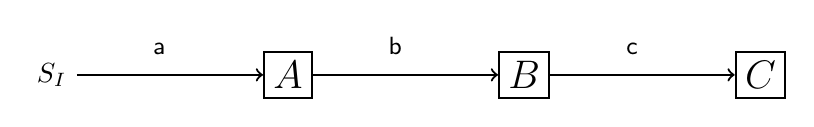
\begin{tikzpicture}[->,auto,node distance=3cm,
			thick,main node/.style={circle,draw,font=\sffamily\Large\bfseries},
			square node/.style={rectangle,draw,font=\sffamily\Large\bfseries}]
			
			\node[] (Invis) [] {$S_I$};
			\node[square node] (A) [right of=Invis] {$A$};
			\node[square node] (B) [right of=A] {$B$};
			\node[square node] (C) [right of=B] {$C$};
			
			\path[every node/.style={font=\sffamily\small}]
			(Invis) edge node [left, label=a] {} (A)
			(A) edge node [left, label=b] {} (B)
			(B) edge node [left, label=c] {} (C);
			\end{tikzpicture}		
		}
	\end{figure}

	The only decomposition for this problem results in the set of un-ordered actions $\{A, B, C\}$.
	If we consider that for the $3!$ linearizations of this set, the only executable one is $A, B, C$. This is impossible to achieve by linearized methods, since ordering either AB before C or C before AB will exclude the solution. 
	Even if we were to produce $k!$ methods for each partially ordered method with $k$ unordered sub-tasks, we would not be able to preserve any solution for this problem.
	
	This proves that the algorithm can remove all solutions, so Algorithm~\ref{alg:Algorithm1} is not complete. Note that incompleteness already follows from complexity theory as it's theoretically impossible to turn an arbitrary undecideable problem into a decidable one.
	Specifically, solutions that require interleaving of sub-tasks will not be preserved, as the example above demonstrates.
	\qed
\end{proof}


We will now see that our algorithm preserves at least one solution as long as Algorithm~\ref{alg:Algorithm1} does not have to break cycles.
\begin{theorem}\label{thm:SpecialCase}
	Given a POHTN planning problem $P$ and TOHTN problem
	$P'$ obtained from $P$ by using Algorithm~\ref{alg:Algorithm1}, if Algorithm~\ref{alg:Algorithm1} did not have to
	cycle-break, then if the solution set of $P$ is non-empty then the solution set of $P'$ will be non-empty as well.
\end{theorem}
\begin{proof}
	Assume that there exists a solution in the PO domain. By using the same decomposition sequence in the linearized domain, we can produce the same set of actions as in the PO solution, but with a linearization of the actions decided by the linearized domain. Assume this sequence is $(a_0, a_1, ..., a_n)$. We then prove by induction over the sequence $(a_0, a_1, ..., a_n)$ that it is executable.
	If $(a_0, a_1, ..., a_n)$ is not executable, that means there exists some action $a_k,  0 < k < n$ that is not executable in the corresponding state. The action $a_k$ could only be non-executable, if one or more of its preconditions was not met. Assume one of these unmet preconditions is for existence of the state variable $A$.
	The action $a_k$ must be executable in some linearization of $\{a_0, ..., a_n\}$, as we assumed it was a PO solution. So there must exist an action $a_i$, $0 < i < n$, that will add A. Actions $a_0$ and $a_k$ must have a shared parent p in a Task Decomposition Tree. So p has subtasks $t_0$ and $t_k$ that are parents of $a_0$ and $a_k$ respectively. 
	
	The linearization of this method would have drawn an ordering $(t_i, t_k)$ due to the way the algorithm defines $prec^{*}, add^{*}$ etc. We are assuming that all methods linearized without conflict, so $(t_i, t_k)$ should not be required. This safely enforces $(a_k, a_0)$ ordering in the final TO plan, meaning $a_0$ is not the first action in the resulting total order imposed by the algorithm. In other words, if $a_k$’s precondition could be met by any action $a_i$, $a_i$ would be ordered in front of it. 
	
	If $a_i$ does not exist then $a_k$ can never be executed for any linearization of $\{a_0, ...a_n\}$, contradicting the assumption that this was a PO solution. Since each action in the solution is executable, the entire sequence is executable linearization of actions produced by decomposition of initial task, i.e. the solution.
	\qed
\end{proof}
 
There are several levels of \enquote{completeness} possible. 
%\begin{enumerate}
	\begin{compactitem}
	\item all solutions remain 
	\item at least one solution remains 
	\item all optimal solutions remain
	\item at least one optimal solution remains 	
	\end{compactitem}
%\end{enumerate}
Given what's proven in Theorem~\ref{thm:notCompleteness} and \ref{thm:SpecialCase}, Algorithm~\ref{alg:Algorithm1} guarantees at least one solution remains, if no cycle-breaking is needed. If cycle-breaking is needed, Algorithm~\ref{alg:Algorithm1} makes no completeness guarantees at all -- it may remove all possible solutions. Finally, Algorithm~\ref{alg:Algorithm1} makes no decisions on any metric of optimality, so obviously cannot guarantee completeness that any optimal solutions remain.
  
  

\begin{theorem}\label{thm:newClass}
	For any problem $P$ that satisfies the criterion for linearization without cycle-breaking, the problem $P'$ obtained from applying the algorithm to $P$ forms a new class of decidable problems.
\end{theorem}
\begin{proof}
	A problem $P'$ obtained from applying Algorithm~\ref{alg:Algorithm1} to any arbitrary $P$ is a totally ordered problem, which are known to be decidable \cite{Alford2015TightHTNBounds}.  
	\qed
\end{proof}

%\begin{theorem}
%	Cycle-breaking is not guaranteed to eliminate solutions.
%\end{theorem}
%\begin{proof}
%	As per proposition 2.1 and 2.2, not all of the preconditions and effects are always needed. Suppose the initial task network consisted of 2 sub-tasks, $t_1, t_2$. If $t_2$ can decompose into an action $a_1$ such that $add(a_1) = A$, and an action $a_2$ such that $del(a_2) = A$,
%	and $t_1$ can decompose into an action $a_3$ with $prec(a_3) = A$
%	$t_2 = {add A, del A}$ and $t_1 = {prec A}$. The rules $\{(add A, prec A), (prec A, del A))\}$ of Algorthm 1
%	require orderings $\{(t_2, t_2), (t_2, t_1), (t_1, t_2)\}$, i.e.
%	Despite a cycle break being needed, this is obviously a solvable problem. Order $t_2$ before $t_1$ for this method.
%	Then when solving decompose $t_2$ to $a_1$ and $t_1$ to $a_3$. This creates a solution. Therefore, it is possible for the algorithm to preserve solutions despite needing cycle-breaking.
%\end{proof}

%%%%  
%\begin{theorem}
%	Given a POHTN planning problem $P = (F, T_P, T_C, \delta, M)$, for a given method $m \in M$, if some task $t \in T_P \cup T_C$ does not have an ordering applied to it by the graph $G$ built in lines 4-11 of Algorithm 1, 
%	then for the TOHTN problem $P'$ obtained from $P$ by using Algorithm 1,
%	the ordering of $t$ will not affect the executability of the final solution.
%	Given a method with all such tasks will cause the solution set of $P$ to equal the solution set of $P'$
%	Or in other words, if a linearization exists at all, it's possible to remove some edges from $G$ in Algorithm 1 to obtain it.
%\end{theorem}
%\begin{proof}
%	Assume that some pair of tasks $t_1, t_2$, Algorithm 1 did not add an ordering between them based off their preconditions and effects. Assume also that the ordering $t_1, t_2$ is executable but $t_2,t_1$ is not, i.e.
%	it matters where they are executed relative to each other.  \newline  \newline
%	This implies that $t_2$ deletes some variable A $t_1$ relies on. But from the definition of Algorithm 1,
%	that would mean that an ordering $(t_1, t_2)$ was created, which contradicts the assumption that there is no ordering between them.
%	Therefore $(t_2, t_1)$ ordering must also be executable. \newline  \newline
%	Thus if some task t has no ordering from the algorithm, it can never matter where it is in relation to any other task.
%	The algorithm will not order it specifically when $(\forall t' \in m, \forall a \in prec(t). a \notin add(t') \land a \notin del(t'))
%	\land  (\forall t' \in m, \forall a \in add(t). a \notin prec(t') \land a \notin del(t')) 
%	\land  (\forall t' \in m, \forall a \in del(t). a \notin add(t') \land a \notin prec(t'))$
%	In other words, the variables that affect t, do not affect other tasks in that method.
%\end{proof}


% \todo{the environments 'definition', 'lemma', 'proposition', 'corollary', 'remark', and 'example' are defined in the LLNCS documentclass as well.}


\section{Empirical Evaluation}
To prove that our technique is beneficial, we conduct a standard empirical evaluation on PO domains and compare the runtime of a state-of-the-art planning system on the original problem vs. the transformed problem. All problems are taken from two benchmark sets prepared for 2020 IPC. The first set\footnote{\url{https://github.com/panda-planner-dev/ipc2020-domains/tree/master/partial-order}} was used in the partially ordered track in the 2020 IPC benchmark, while the second set\footnote{\url{https://github.com/panda-planner-dev/domains/tree/master/partial-order}} went un-used for various reasons. However, the second set still contains valid POHTN problems, so we include it here as well. Each problem has the standard IPC time limit of 30 minutes. Where grounding and pre-processing is needed, the time to do this is included as part of the 'solving' time required. Since the pre-processing may \emph{potentially} remove all solutions, where the planning system can prove that the pre-processing renders a problem unsolvable, we use the remaining time to solve the original problem.


\subsubsection{Hardware and Planning Systems}
The empirical evaluation was conducted on a machine with 30GiB of memory and 4 vCPUs, each with 2 GiB RAM, for a total of 8 GiB RAM.  We use the $panda_{\pi}$ solver \cite{progressionsearchJAIR20} \cite{useClassicalHeuristicIJCAI19} \cite{useClassicalHuristicICAPS18} on the configuration of Greedy best first search with  visited lists. We try this search with 4 different RC-heuristics: FF \cite{FF}, Add \cite{Add}, Filter \cite{useClassicalHuristicICAPS18} and Landmark-cut \cite{LM-Cut}.

We compare the performance of these 4 planner settings on the original problem and the pre-processed problem.
We also try the Lilotane planner \cite{Lilotane}, which is specialised for TOHTN problems. 
%VCPUs  : 4 \newline
%Memory : 8GB, OR 8192(MB) \newline
%Disk   : 30GB \newline
%RAM per VCPU; 2GB \newline
%CPU Shares: 256 \newline
  
\subsection{Results}

\begin{figure}
	\floatbox[{\capbeside\thisfloatsetup{capbesideposition={left,center},capbesidewidth=6cm}}]{figure}[\FBwidth]
	{\caption{Percentage of problems for which linearized problems is faster to solve, for problems that took at least $\mathit{x}$ seconds to solve, with $\mathit{x}$  being the value on the x-axis. \\ \label{faster}}}
	{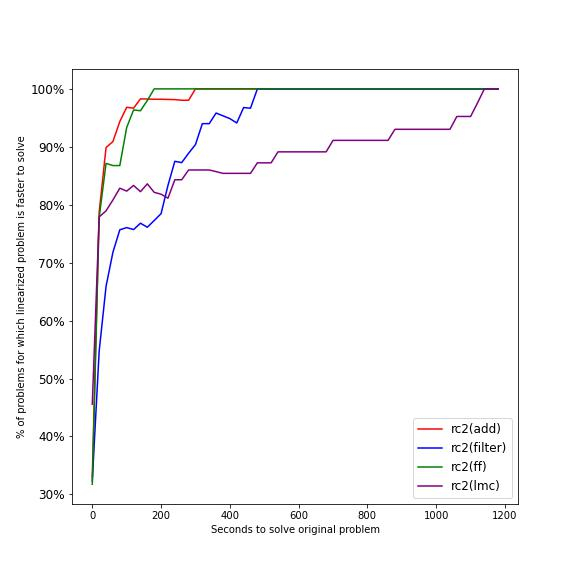
\includegraphics[width=5cm]{figures/faster_to_solve_m.jpg}}

\end{figure}


\begin{table} 
\setlength{\tabcolsep}{2.5pt} 
\caption{IPC score, with and without pre-processing, for all planners. If any problems in that domain were proven unsolvable by TO, a number in brackets beside domain name shows how many.} \label{tabIPC} 
 \scalebox{0.9}{ 
 \begin{tabular}{lccccccccccccccccccl} 
\toprule 
  && \multicolumn{2}{c}{RC\textsuperscript{add}} & \multicolumn{2}{c}{RC\textsuperscript{Filter}} & \multicolumn{2}{c}{RC\textsuperscript{FF}} & \multicolumn{2}{c}{RC\textsuperscript{LM-Cut}} & \multicolumn{2}{c}{Lilotane} \\ 
\cmidrule(lr){3-4} \cmidrule(lr){5-6} \cmidrule(lr){7-8} \cmidrule(lr){9-10} \cmidrule(lr){11-12}  
 & max &PO & TO & PO & TO & PO & TO & PO &\multicolumn{2}{c}{ TO  } \\ 
\midrule 
Barman-BDI & 1 & 0.08 & \textbf{0.4} & 0.07 & \textbf{0.34} & 0.07 & \textbf{0.36} & 0.05 & \textbf{0.22} &\multicolumn{2}{c}{ \textbf{0.66}  } \\ 
 Monroe Fully Observ. (2) & 1 & \textbf{0.56} & 0.45 & \textbf{0.31} & 0.3 & \textbf{0.46} & 0.41 & \textbf{0.22} & 0.18 &\multicolumn{2}{c}{ 0.07  } \\ 
 Monroe Part. Observ. (2) & 1 & \textbf{0.31} & 0.25 & \textbf{0.13} & 0.11 & \textbf{0.31} & 0.26 & \textbf{0.17} & 0.14 &\multicolumn{2}{c}{ 0.0  } \\ 
PCP (17) & 1 & \textbf{0.82} & \textbf{0.82} & \textbf{0.82} & \textbf{0.82} & \textbf{0.82} & \textbf{0.82} & \textbf{0.82} & \textbf{0.82} &\multicolumn{2}{c}{ 0.0  } \\ 
Rover & 1 & 0.29 & \textbf{0.95} & 0.14 & \textbf{0.52} & 0.2 & \textbf{0.78} & 0.16 & \textbf{0.48} &\multicolumn{2}{c}{ \textbf{0.98}  } \\ 
Satellite & 1 & 0.91 & \textbf{1.0} & 0.76 & \textbf{1.0} & 0.99 & \textbf{1.0} & 0.89 & \textbf{0.99} &\multicolumn{2}{c}{ \textbf{1.0}  } \\ 
SmartPhone (1) & 1 & \textbf{0.71} & \textbf{0.71} & 0.69 & \textbf{0.71} & \textbf{0.71} & \textbf{0.71} & \textbf{0.71} & \textbf{0.71} &\multicolumn{2}{c}{ \textbf{0.71}  } \\ 
Transport & 1 & 0.24 & \textbf{0.61} & 0.04 & \textbf{0.05} & 0.27 & \textbf{0.32} & 0.12 & \textbf{0.2} &\multicolumn{2}{c}{ \textbf{0.71}  } \\ 
UM-Translog (1) & 1 & \textbf{1.0} & \textbf{1.0} & \textbf{1.0} & \textbf{1.0} & \textbf{1.0} & \textbf{1.0} & \textbf{1.0} & \textbf{1.0} &\multicolumn{2}{c}{ 0.95  } \\ 
Woodworking (2)& 1 & 0.38 & \textbf{0.58} & 0.2 & \textbf{0.41} & 0.36 & \textbf{0.57} & 0.27 & \textbf{0.39} &\multicolumn{2}{c}{ 0.47  } \\ 
\midrule 
 Monroe & 1 & \textbf{0.77} & 0.69 & \textbf{0.5} & 0.47 & \textbf{0.75} & 0.71 & \textbf{0.53} & \textbf{0.53} &\multicolumn{2}{c}{ 0.46  } \\ 
SmartPhone (1) & 1 & \textbf{0.71} & \textbf{0.71} & 0.69 & \textbf{0.71} & \textbf{0.71} & \textbf{0.71} & \textbf{0.71} & \textbf{0.71} &\multicolumn{2}{c}{ \textbf{0.71}  } \\ 
Zenotravel & 1 & \textbf{1.0} & \textbf{1.0} & 0.63 & \textbf{1.0} & \textbf{1.0} & \textbf{1.0} & 0.83 & \textbf{1.0} &\multicolumn{2}{c}{ \textbf{1.0}  } \\ 
\midrule
Total IPC score & 13 & 7.8 & \textbf{9.2} & 6.0 & \textbf{7.5} & 7.7 & \textbf{8.7} & 6.5 & \textbf{7.4} &\multicolumn{2}{c}{ 7.7  } \\ 
\bottomrule 
 \end{tabular} 
} 
\end{table} 

\begin{table} 
\setlength{\tabcolsep}{2.5pt} 
\caption{Coverage, with and without pre-processing, for all planners. If any problems in that domain were proven unsolvable by TO, a number in brackets beside domain name shows how many.}\label{tabcoverage} 
 \scalebox{0.9}{ 
 \begin{tabular}{lccccccccccccccccccl} 
\toprule 
  && \multicolumn{2}{c}{RC\textsuperscript{add}} & \multicolumn{2}{c}{RC\textsuperscript{Filter}} & \multicolumn{2}{c}{RC\textsuperscript{FF}} & \multicolumn{2}{c}{RC\textsuperscript{LM-Cut}} & \multicolumn{2}{c}{Lilotane} \\ 
\cmidrule(lr){3-4} \cmidrule(lr){5-6} \cmidrule(lr){7-8} \cmidrule(lr){9-10} \cmidrule(lr){11-12}  
 & max &PO & TO & PO & TO & PO & TO & PO &\multicolumn{2}{c}{ TO  } \\ 
\midrule 
Barman-BDI & 20 & 3 & \textbf{10} & 3 & \textbf{10} & 3 & \textbf{10} & 2 & \textbf{9} &\multicolumn{2}{c}{ \textbf{16}  } \\ 
 Monroe Fully Observ. (2) & 25 & \textbf{25} & \textbf{25} & 18 & \textbf{25} & 22 & \textbf{25} & 15 & \textbf{16} &\multicolumn{2}{c}{ 6  } \\ 
 Monroe Part. Observ. (2) & 24 & \textbf{14} & \textbf{14} & \textbf{7} & \textbf{7} & 14 & \textbf{15} & \textbf{10} & \textbf{10} &\multicolumn{2}{c}{ 0  } \\ 
PCP (17) & 17 & \textbf{14} & \textbf{14} & \textbf{14} & \textbf{14} & \textbf{14} & \textbf{14} & \textbf{14} & \textbf{14} &\multicolumn{2}{c}{ 0  } \\ 
Rover & 20 & 6 & \textbf{20} & 4 & \textbf{14} & 4 & \textbf{19} & 4 & \textbf{14} &\multicolumn{2}{c}{ \textbf{20}  } \\ 
Satellite & 25 & 24 & \textbf{25} & 22 & \textbf{25} & \textbf{25} & \textbf{25} & 24 & \textbf{25} &\multicolumn{2}{c}{ \textbf{25}  } \\ 
SmartPhone (1) & 7 & \textbf{5} & \textbf{5} & \textbf{5} & \textbf{5} & \textbf{5} & \textbf{5} & \textbf{5} & \textbf{5} &\multicolumn{2}{c}{ \textbf{5}  } \\ 
Transport & 40 & 12 & \textbf{28} & \textbf{2} & \textbf{2} & 13 & \textbf{14} & 7 & \textbf{12} &\multicolumn{2}{c}{ \textbf{31}  } \\ 
UM-Translog (1) & 22 & \textbf{22} & \textbf{22} & \textbf{22} & \textbf{22} & \textbf{22} & \textbf{22} & \textbf{22} & \textbf{22} &\multicolumn{2}{c}{ 21  } \\ 
Woodworking (2) & 30 & 13 & \textbf{19} & 7 & \textbf{15} & 12 & \textbf{20} & 9 & \textbf{15} &\multicolumn{2}{c}{ 15  } \\ 
\midrule 
 Monroe & 100 & 96 & \textbf{100} & 79 & \textbf{88} & 92 & \textbf{100} & 81 & \textbf{90} &\multicolumn{2}{c}{ 83  } \\ 
SmartPhone (1) & 7 & \textbf{5} & \textbf{5} & \textbf{5} & \textbf{5} & \textbf{5} & \textbf{5} & \textbf{5} & \textbf{5} &\multicolumn{2}{c}{ \textbf{5}  } \\ 
Zenotravel & 5 & \textbf{5} & \textbf{5} & \textbf{5} & \textbf{5} & \textbf{5} & \textbf{5} & \textbf{5} & \textbf{5} &\multicolumn{2}{c}{ \textbf{5}  } \\ 
\midrule 
 Coverage & 342 & 244 & \textbf{292} & 193 & \textbf{237} & 236 & \textbf{279} & 203 & \textbf{242} &\multicolumn{2}{c}{ 232  } \\ 
Norm. coverage & 13 & 8.94 & \textbf{10.67} & 7.57 & \textbf{9.17} & 8.71 & \textbf{10.34} & 7.81 & \textbf{9.16} &\multicolumn{2}{c}{ 8.53  } \\ 
\bottomrule 
 \end{tabular} 
} 
\end{table} 

% 'UM-Translog': 1, 'Monroe-Fully-Observable': 2, 'Woodworking': 2, 'Monroe-Partially-Observable': 2, 'PCP': 17, 'SmartPhone': 1}
 
\begin{figure}[t]
	\caption{Comparison of time to solve PO and TO problems, for each $panda_{\pi}$ setting} \label{RuntimevsSolved}
	\begin{subfigure}{6cm}
		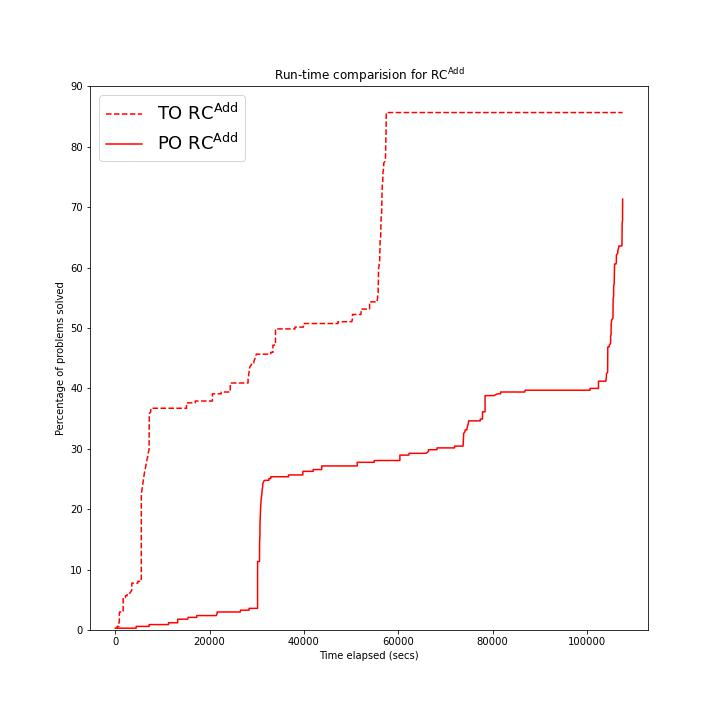
\includegraphics[width=5cm]{figures/Runtime comparisionRC(Add).jpg}	
		\caption{Using heuristic RC\textsuperscript{add}}	
	\end{subfigure}
	\begin{subfigure}{6cm}
		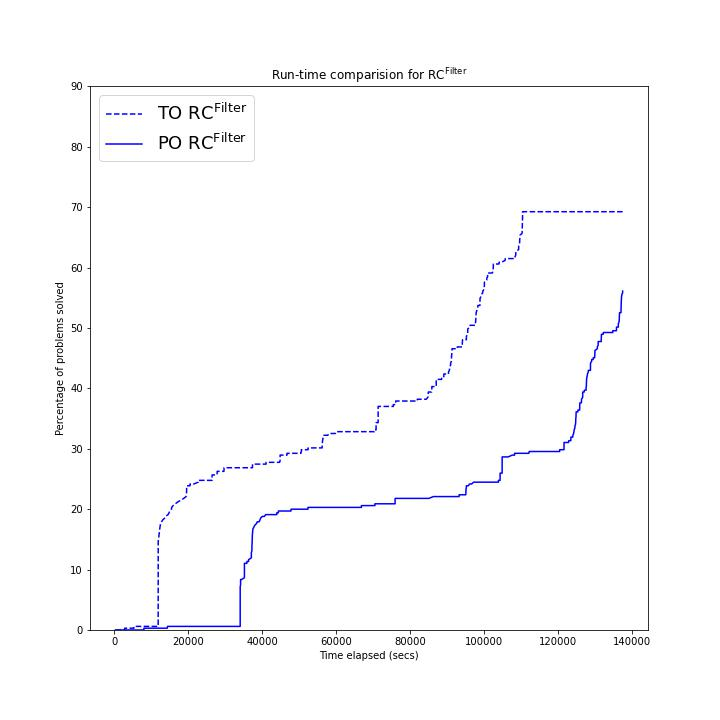
\includegraphics[width=5cm]{figures/Runtime comparisionRC(Filter).jpg}	
		\caption{Using heuristic RC\textsuperscript{Filter}}
	\end{subfigure}

	\begin{subfigure}{6cm}
		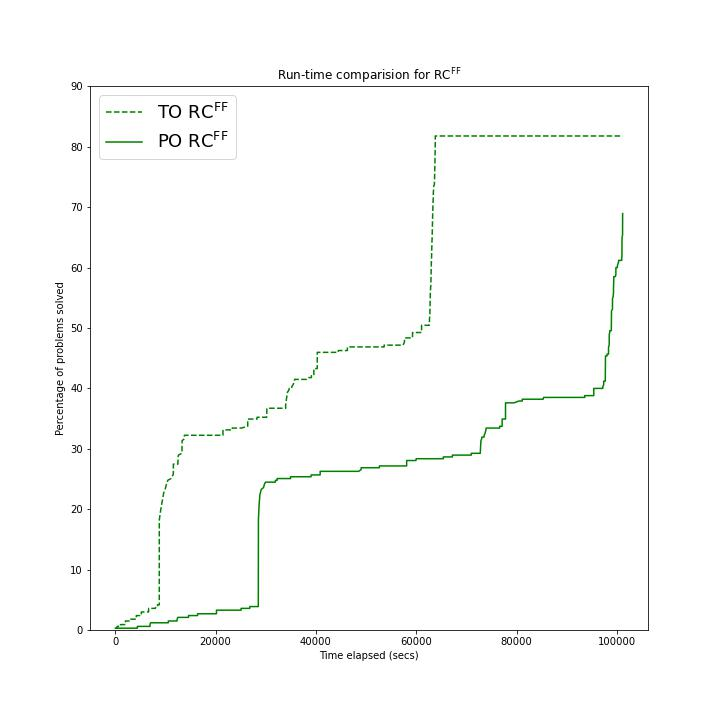
\includegraphics[width=5cm]{figures/Runtime comparisionRC(FF).jpg}	
		\caption{Using heuristic RC\textsuperscript{FF}}	
	\end{subfigure}
	\begin{subfigure}{6cm}
		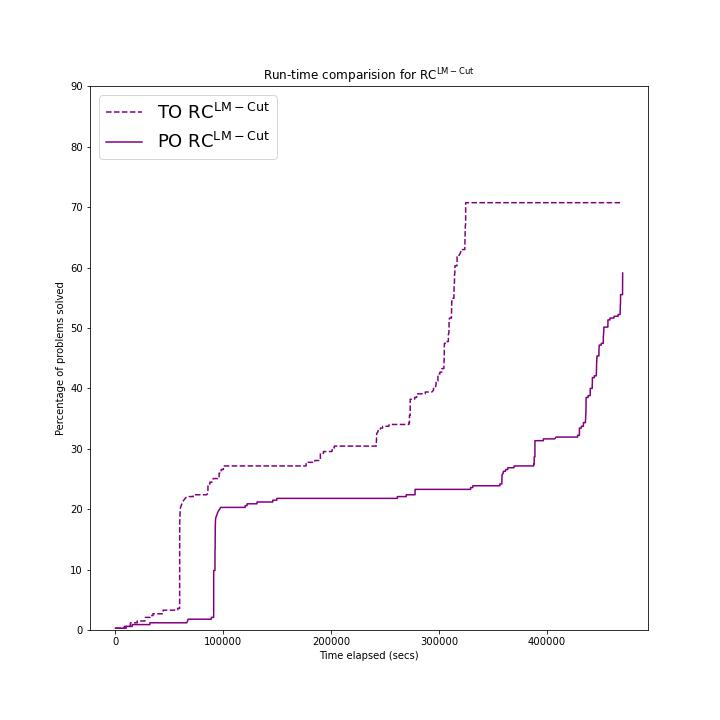
\includegraphics[width=5cm]{figures/Runtime comparisionRC(LM-Cut).jpg}
		\caption{Using heuristic RC\textsuperscript{LM-Cut}}		
	\end{subfigure}
\end{figure}

 
\subsection{Analysis}

Table~\ref{tabIPC} and \ref{tabcoverage} shows that the IPC score and coverage when pre-processing is overall significantly better than when not using pre-processing. 

However in some domains there is minimal gain, if any at all. This seems to be because some domains are dominated by small problems. E.g.\ 14 of the 17 PCP problems take less than 0.5 seconds to solve. For very small problems, the pre-processing still takes time, but very little improvement can be gained in the actual solving time. In fact, a second of pre-processing time for a problem that only takes a few seconds to solve will worsen IPC score. 

On the other hand, big problems experience significant improvement, enough to make problems solvable within the time limit where they were previously too memory or time intensive. We can see that difference in domains like Rover and Barman-BDI, where there is significant space to improve on coverage/speed.
 
\begin{table}[t] 
	\setlength{\tabcolsep}{2.5pt} 
\caption{With re-run policy}\label{tabsummary2} 
\scalebox{0.85}{
 \begin{tabular}{lccccccl} 
\toprule 
&   & Solved & Out of Memory & Timeout & Unsolvable &  \\ 
\midrule
  \multirow{3}*{RC\textsuperscript{add}}& TO & 287 & 27 & 21 & 0  \\ 
& PO & 239 & 65 & 31 & 0  \\ 
& Either & 287 & 72 & 40 & 0  \\ 
\midrule 
 \multirow{3}*{RC\textsuperscript{Filter}}& TO & 232 & 85 & 18 & 0  \\ 
& PO & 188 & 115 & 32 & 0  \\ 
& Either & 232 & 125 & 35 & 0  \\ 
\midrule 
 \multirow{3}*{RC\textsuperscript{FF}}& TO & 274 & 41 & 20 & 0  \\ 
& PO & 231 & 76 & 28 & 0  \\ 
& Either & 274 & 85 & 37 & 0  \\ 
\midrule 
 \multirow{3}*{RC\textsuperscript{LM-Cut}}& TO & 237 & 6 & 92 & 0  \\ 
& PO & 198 & 11 & 126 & 0  \\ 
& Either & 237 & 12 & 126 & 0  \\ 
\bottomrule 
 \end{tabular} 
}
\end{table} 

\begin{table}[t]
	\setlength{\tabcolsep}{2.5pt} 
\caption{Without re-run policy}\label{tabsummary1} 
\scalebox{0.85}{
 \begin{tabular}{lccccccl} 
\toprule 
&   & Solved & Out of Memory & Timeout & Unsolvable &  \\ 
\midrule
\multirow{3}*{RC\textsuperscript{add}}& TO & 266 & 24 & 20 & 25  \\ 
& PO & 239 & 65 & 31 & 0  \\ 
& Either & 287 & 72 & 40 & 25  \\ 
\midrule 
 \multirow{3}*{RC\textsuperscript{Filter}}& TO & 212 & 80 & 18 & 25  \\ 
& PO & 188 & 115 & 32 & 0  \\ 
& Either & 232 & 125 & 35 & 25  \\ 
\midrule 
 \multirow{3}*{RC\textsuperscript{FF}}& TO & 253 & 38 & 19 & 25  \\ 
& PO & 231 & 76 & 28 & 0  \\ 
& Either & 274 & 85 & 37 & 25  \\ 
\midrule 
 \multirow{3}*{RC\textsuperscript{LM-Cut}}& TO & 217 & 2 & 91 & 25  \\ 
& PO & 198 & 11 & 126 & 0  \\ 
& Either & 237 & 12 & 126 & 25  \\ 
\midrule 
Lilotane & TO & 227 & 108 & 0 & 0  \\ 
\bottomrule 
 \end{tabular}
} 
\end{table} 


Table~\ref{tabsummary1} and Table~\ref{tabsummary2} summarises the results of our empirical evaluation on the IPC 2020 benchmarks. The \enquote{unsolvable} columns refer to problems that the solver determined to have no solutions. Lilotane \cite{Lilotane}, the runner-up for the totally ordered track in the 2020 IPC competition, cannot prove that a problem is unsolvable, and thus can't use a re-run policy, unlike the $panda_{\pi}$ planner.
Note that Lilotane wants a lifted representation,
but a grounded representation was used here, to its disadvantage.

The PCP domain in particular was rendered unsolvable for all instances.  In Table~\ref{tabIPC} and Table~\ref{tabcoverage}, $\text{PCP}^{17}$ indicates that 17 PCP problems were unsolvable. So all 14 problems \enquote{solved} in the TO context was from re-running the planner on the original problem using the remaining time. Incidentally, the exact same problems were proven unsolvable for all planners.

The PCP domain defines the post-correspondence problem, which is known to be undecidable. Totally ordered HTN planning problems are always decidable \cite{LanguageClassificationPlanning}, meaning it's a direct consequence that these problem instances are unsolvable without task interleaving. In this specific case, the PCP problems designed for the IPC benchmark are known to be unsolvable without interleaving \cite{PCPDomain}. Table~\ref{tabsummary2} shows the results on the default setting, when allowing the planner to try solving the original problem as a back-up plan when the linearized problem fails. Lilotane is excluded from Table~\ref{tabsummary2} as it cannot prove a problem is unsolvable, and so cannot use the re-run policy. instead. Table~\ref{tabsummary1} shows results without the default back-up strategy.  % the planner moves on to the next problem immediately after the linearized approach for a problem fails.
%  This means that if we could convert such that it retained a solution, we would be turning an undecidable problem into a decidable one -- in other words impossible. A totally ordered problem just does not have the expressive power.


From Table ~\ref{tabsummary2} and \ref{tabsummary1} we can see that this processing means that many more problems can be solved in the time limit, where previously they were too computation-intensive, and very few problems (primarily problems for which interleaving is required for all solutions) become unsolvable due to the transformation. Despite the fact that none of the instances can be linearized without cycle-breaking, only 25/274 of linearized problems are unsolvable, 17 of which are from the PCP domain, where a solvable linearization does not exist.


\section{Conclusion}
Though it's impressive performance on a range of domains is good news, the success of this approach on the IPC benchmark ultimately hinges on the relative lack of unsolvable problems --
e.g. PCP problems in the ICAPS benchmark. When the pre-processed domain eliminates all solutions, significant time is wasted in proving this. Fortunately, the IPC benchmark covers a wide variety of domains, so the performance of the pre-processing is hopefully indicative of good performance in other problems as well. Ultimately, it's also an undecidable problem to detect when a problem cannot be converted to TOHTN representation (as that would be solving whether the problem is undecidable), so no perfect solution exists.
% . For example, a simple machine learning model that learns when the pre-processing step could be applied, by analysing some basic features of the problem, such as size of the problem, structure of the Task Decomposition Graph, etc, could further improve, and is of interest in further work.
\section{Further Work}
Given that HyperTensioN \cite{hypertension} and Lilotane \cite{Lilotane}, planning systems that work on \emph{lifted} totally ordered problems, and rely significantly on lifted input for their efficiency, it would be of interest to generalise this technique to produce lifted domains, so that HyperTensioN and Lilotane can solve the linearized problem more efficiently. For another, the success of this solution was, as stated before, in part due to the relatively few undecidable problems in the benchmark set. A heuristic to decide whether or not to pre-process, so that we can reduce the case where the planning system attempts to solve an unsolvable problem might allow this procedure to generalise better in less favourable circumstances. 

%A less naive procedure for approximating preconditions and effects for compound tasks, allowing stronger assumptions to be made when linearizing, may also be of interest. 
	
%The additional processing time is within the same order of time as the time needed for grounding and a tiny fraction of the overall time $\sim$   We compare the ratio of (Grounding + Pre-processing time + TO solve time) to (Grounding + PO solve time), as those are the steps needed to solve the respective problems. The average solve time for the TO problem is ?? percent of the PO problem, for all problems. Difference in reduction of total solving time influenced most by ? (e.g. domain, recursiveness of problem, percentage of linearizable methods, etc)

%\subsubsection{Acknowledgements} Please place your acknowledgments at
%the end of the paper, preceded by an unnumbered run-in heading (i.e.
%3rd-level heading).

%
% ---- Bibliography ----
%
% BibTeX users should specify bibliography style 'splncs04'.
% References will then be sorted and formatted in the correct style.
%
\bibliographystyle{splncs04}
\bibliography{bib}
% %\bibitem{ref_article1}
% %Author, F.: Article title. Journal \textbf{2}(5), 99--110 (2016)

% %\bibitem{ref_lncs1}
% %Author, F., Author, S.: Title of a proceedings paper. In: Editor,
% %F., Editor, S. (eds.) CONFERENCE 2016, LNCS, vol. 9999, pp. 1--13.
% %Springer, Heidelberg (2016). \doi{10.10007/1234567890}

% %\bibitem{ref_book1}
% %Author, F., Author, S., Author, T.: Book title. 2nd edn. Publisher,
% %Location (1999)

% %\bibitem{ref_proc1}
% %Author, A.-B.: Contribution title. In: 9th International Proceedings
% %on Proceedings, pp. 1--2. Publisher, Location (2010)

% %\bibitem{ref_url1}
% %LNCS Homepage, \url{http://www.springer.com/lncs}. Last accessed 4
% %Oct 2017
% \end{thebibliography}
\end{document}
